\section*{29. Скалярный потенциал магнитного поля.}
 
Согласно первому уравнению Максвелла в тех местах, где есть плотность тока, ротор вектора напряженности не равен нулю и поле имеет вихревой характер. В тех областях, где плотность тока равна нулю ($\delta =0$) $\mathrm{rot}\vec{H}$  , магнитное поле можно рассматривать как потенциальное



\noindent
\begin{minipage}[c]{0.3\textwidth} % Левая часть: изображение
    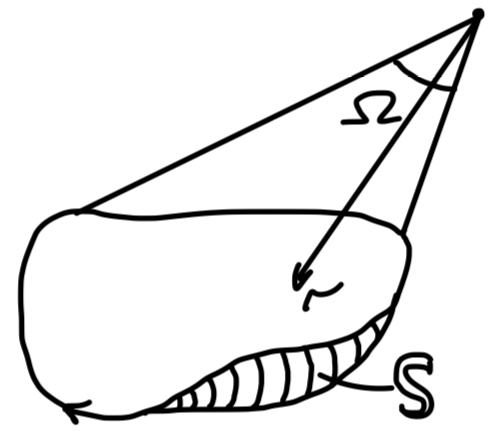
\includegraphics[width=\textwidth]{im/64.png}{} % Ваше изображение
\end{minipage}%
\hfill
\begin{minipage}[c]{0.55\textwidth} % Правая часть: текст
    \( \mathrm{rot}\vec{H}=\frac{4\pi}{c}\vec{j}   \) 
    
    \( \psi: \vec{H}=-\grad \psi \)
    
    \( \psi = \frac{I}\Omega  \) 

    \( \Omega =\underset{S}{\iint}\frac{d\vec{S}}{r^2} \frac{\vec{r}}{r}   \) 
\end{minipage}
\[\text{ }\]
\noindent
\begin{minipage}[c]{0.4\textwidth} % Левая часть: изображение
    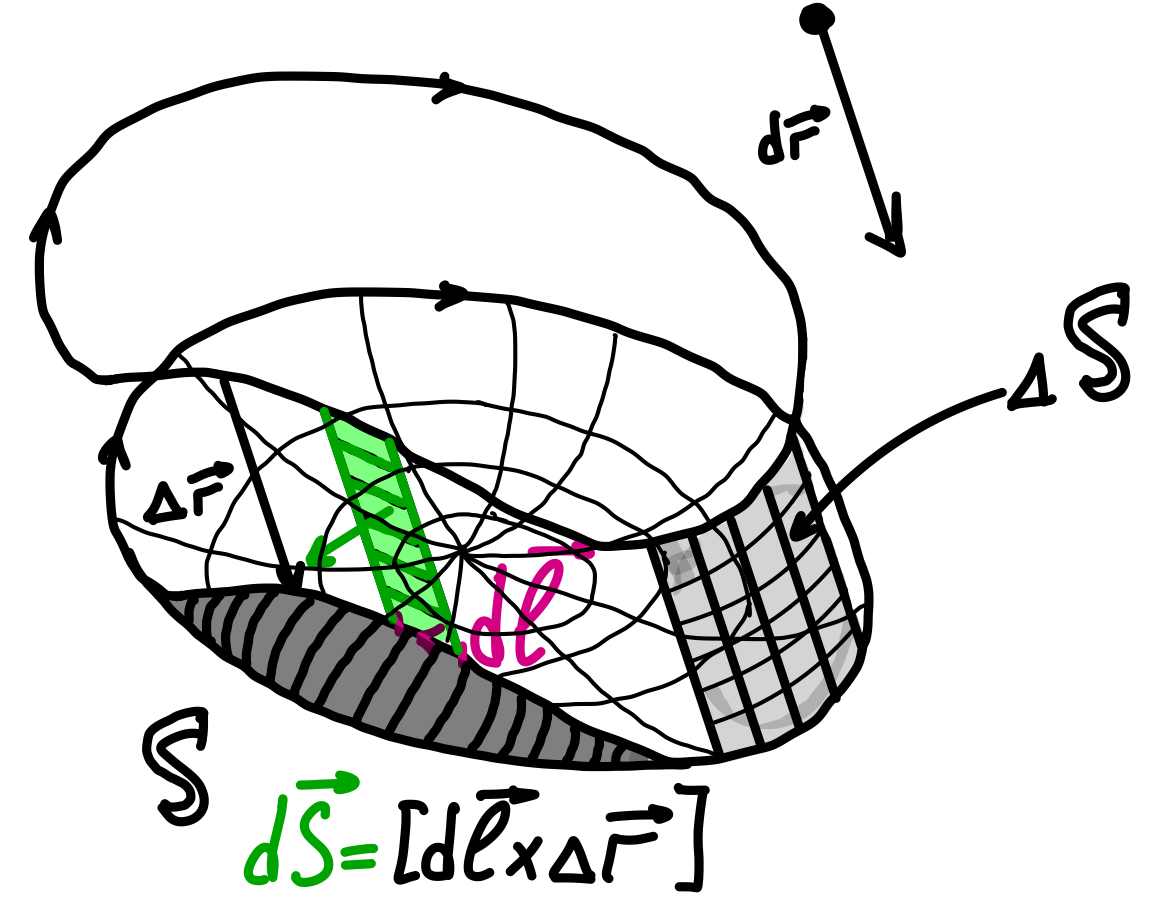
\includegraphics[width=\textwidth]{im/65.png}{} % Ваше изображение
\end{minipage}%
\hfill
\begin{minipage}[c]{0.55\textwidth} % Правая часть: текст
    \( \Delta\Omega =(\grad\Omega)\Delta \vec{r} \) 

    \( \Omega= \underset{S}{\iint}\frac{\vec{r}}{r^3}d\vec{S};\quad \Omega+\Delta\Omega =\underset{S+\Delta S}{\iint} \frac{\vec{r}}{r^3}d\vec{S};  \)
    
    \( \Delta\Omega= \underset{\Delta S}{\iint} \frac{\vec{r}}{r^3}= \oint \left( \frac{\vec{r}}{r^3}[d\vec{l}\times \Delta\vec{r}]  \right)=  \)

    \(\qquad = \Delta\vec{r} \oint \left[ \frac{\vec{r}}{r^3}\times d\vec{l}  \right] \Rightarrow   \) 
\end{minipage}

\[
\Rightarrow \grad\Omega=\oint \left[ \frac{\vec{r}}{r^3}\times d\vec{l}  \right]
\]

\[
\vec{H}=\frac{I}{c}\oint \left[ \frac{d\vec{l} \times \vec{r}}{r^3}  \right] = -\frac{I}{c} \grad \psi
\]